\documentclass{beamer}
\usetheme{Copenhagen}
\usepackage[utf8]{inputenc}
\usepackage[brazil]{babel}  % Pacote
\usepackage{mflogo}
\usepackage{listings}
\usepackage{caption}
\author{Amadeus Folego}
\title{\LaTeX\ em aplicações Rails}
\date{}
\institute{
  \begin{tabular}{c c}        
    {\em www} & \url{http://badosu.com}\\
    {\em email} & \url{amadeusfolego@gmail.com}
  \end{tabular}
}
\begin{document}
  \begin{frame}[plain] 
    \titlepage
  \end{frame}
  \begin{frame}{Apresentação}
  \end{frame}
  \begin{frame}{Don Knuth}
    \begin{columns}[c]
      \column{.2\textwidth}
        \begin{figure}[t]
          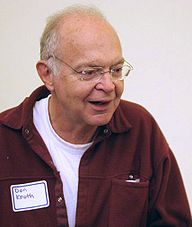
\includegraphics[width=\columnwidth]{192px-KnuthAtOpenContentAlliance}
          \caption*{\scriptsize Donald Ervin Knuth}
        \end{figure}
      \column{.8\textwidth}
        \begin{itemize}
          \item "Pai" da análise de algoritmos \pause
          \item Números Surreais /w John Conway \pause
          \item Livros \pause
            \begin{itemize}
              \item {\em The Art of Computer Programming (TAOCP) - 1969} \pause
              \item {\em Concrete Mathematics - 1970} \pause 
              \begin{itemize}
                \item {\scriptsize Um dólar hexadecimal por cada erro técnica, histórica, tipográfica ou politicamente incorreto \ (\$ 2.56)} \pause 
              \end{itemize}
            \end{itemize}
          \item \TeX\ e \MF
        \end{itemize}
    \end{columns}
  \end{frame}
  \begin{frame}{\LaTeX\ ?}
    Por quê \LaTeX?\\\pause
    \begin{itemize}
      \item{\fontfamily{cmr}\selectfont Excelência tipográfica (Computer Modern)\pause
        \begin{itemize}
          \item Knuth, ao receber a prévia da segunda edição do {\em Concrete Mathematics}\pause
        \end{itemize}}
      \item \TeX\ $\implies$ \LaTeX\ \ \ \scriptsize{1976 Knuth - 1980's Leslie Lamport}\pause
      \item Um dos primeiros projetos de software livre\pause
      \item Comunidade enorme (praticamente a maioria dos cientistas), milhares de pacotes e tipos de documento
    \end{itemize}
  \end{frame}
  \begin{frame}{Capacidades}
    \onslide<1>{$ \rightarrow $} Conteúdo sobre formatação\\\pause
    \onslide<2>{$ \rightarrow $} Extremamente extensivo\\\pause
    \onslide<3>{$ \rightarrow $} É apenas texto\\\pause
    \onslide<4->{$ \rightarrow $} Expressões matemáticas\\\pause 
      $$ \oint_{D} B\cdot n\ dS = 0 $$ 
    \onslide<5>\pause\href{doc/rogers}{\beamerbutton{Exemplo}}
  \end{frame}
  \lstset{extendedchars=false,language=tex,basicstyle=\ttfamily}
  \begin{frame}{Pedaços de código}
    \lstinputlisting[firstline=1,lastline=8,title=Declaração]{presentation.tex}
  \end{frame}
  \begin{frame}{Pedaços de código}
    \lstinputlisting[firstline=17,lastline=21,title=Comandos]{presentation.tex}
  \end{frame}
  \begin{frame}{Desvantagens}
    \onslide<1->{ $ \rightsquigarrow $ } Exige muitas dependências\\\pause
    \onslide<2->{ $ \rightsquigarrow $ } É compilado\\\pause
    \onslide<3> { $ \rightsquigarrow $ } Barreira inicial de aprendizado
  \end{frame}
  \begin{frame}{Motivação} 
    \onslide<1>{$ \nabla $} Aplicações web, geração de documentos\\\pause
    \onslide<2>{$ \nabla $} Latex é apenas texto\\\pause
    \onslide<3>{$ \nabla $} Quantidade enorme de tipos de documento\\
  \end{frame}
  \begin{frame}{Fim} 
    \begin{center} \fontfamily{cmr}\selectfont \Huge FIM \end{center}
  \end{frame}
  \begin{frame}{Mão na massa} 
    \begin{center} \href{https://github.com/jacott/rails-latex}{\beamergotobutton{rails-latex}} \end{center}
  \end{frame}
  \begin{frame}[plain] 
    \titlepage
  \end{frame}
\end{document}
